\section{System Model and Application Profiles}

% A complementary method to improve scalability is through judicious
% allocation of cloudlet resources among concurrent application
% services. 

Resource allocation has been well explored in many contexts
of computer systems, including operating system, networks, real-time
systems, and cloud data centers.  While these prior efforts can
provide design blueprints for cloudlet resource allocation, the
characteristics of edge-native applications emphasize unique design
challenges.

The ultra-low application latency requirements of edge-native
applications are at odds with large queues often used to maintain high
resource utilization of scarce resources.  Even buffering a small
number of requests may result in end-to-end latencies that are several
multiples of processing delays, hence exceeding acceptable latency
thresholds.  On the other hand, when using short queues, accurate
estimations of throughput, processing, and networking delay are vital
to enable efficient use of cloudlet resources.  However, sophisticated
computer vision processing represents a highly variable computational
workload, even on a single stream. For example, as shown in
Figure~\ref{fig:lego-dag}, the processing pipeline for LEGO has many
exits, resulting in highly variable execution times.

\begin{figure}
\centering
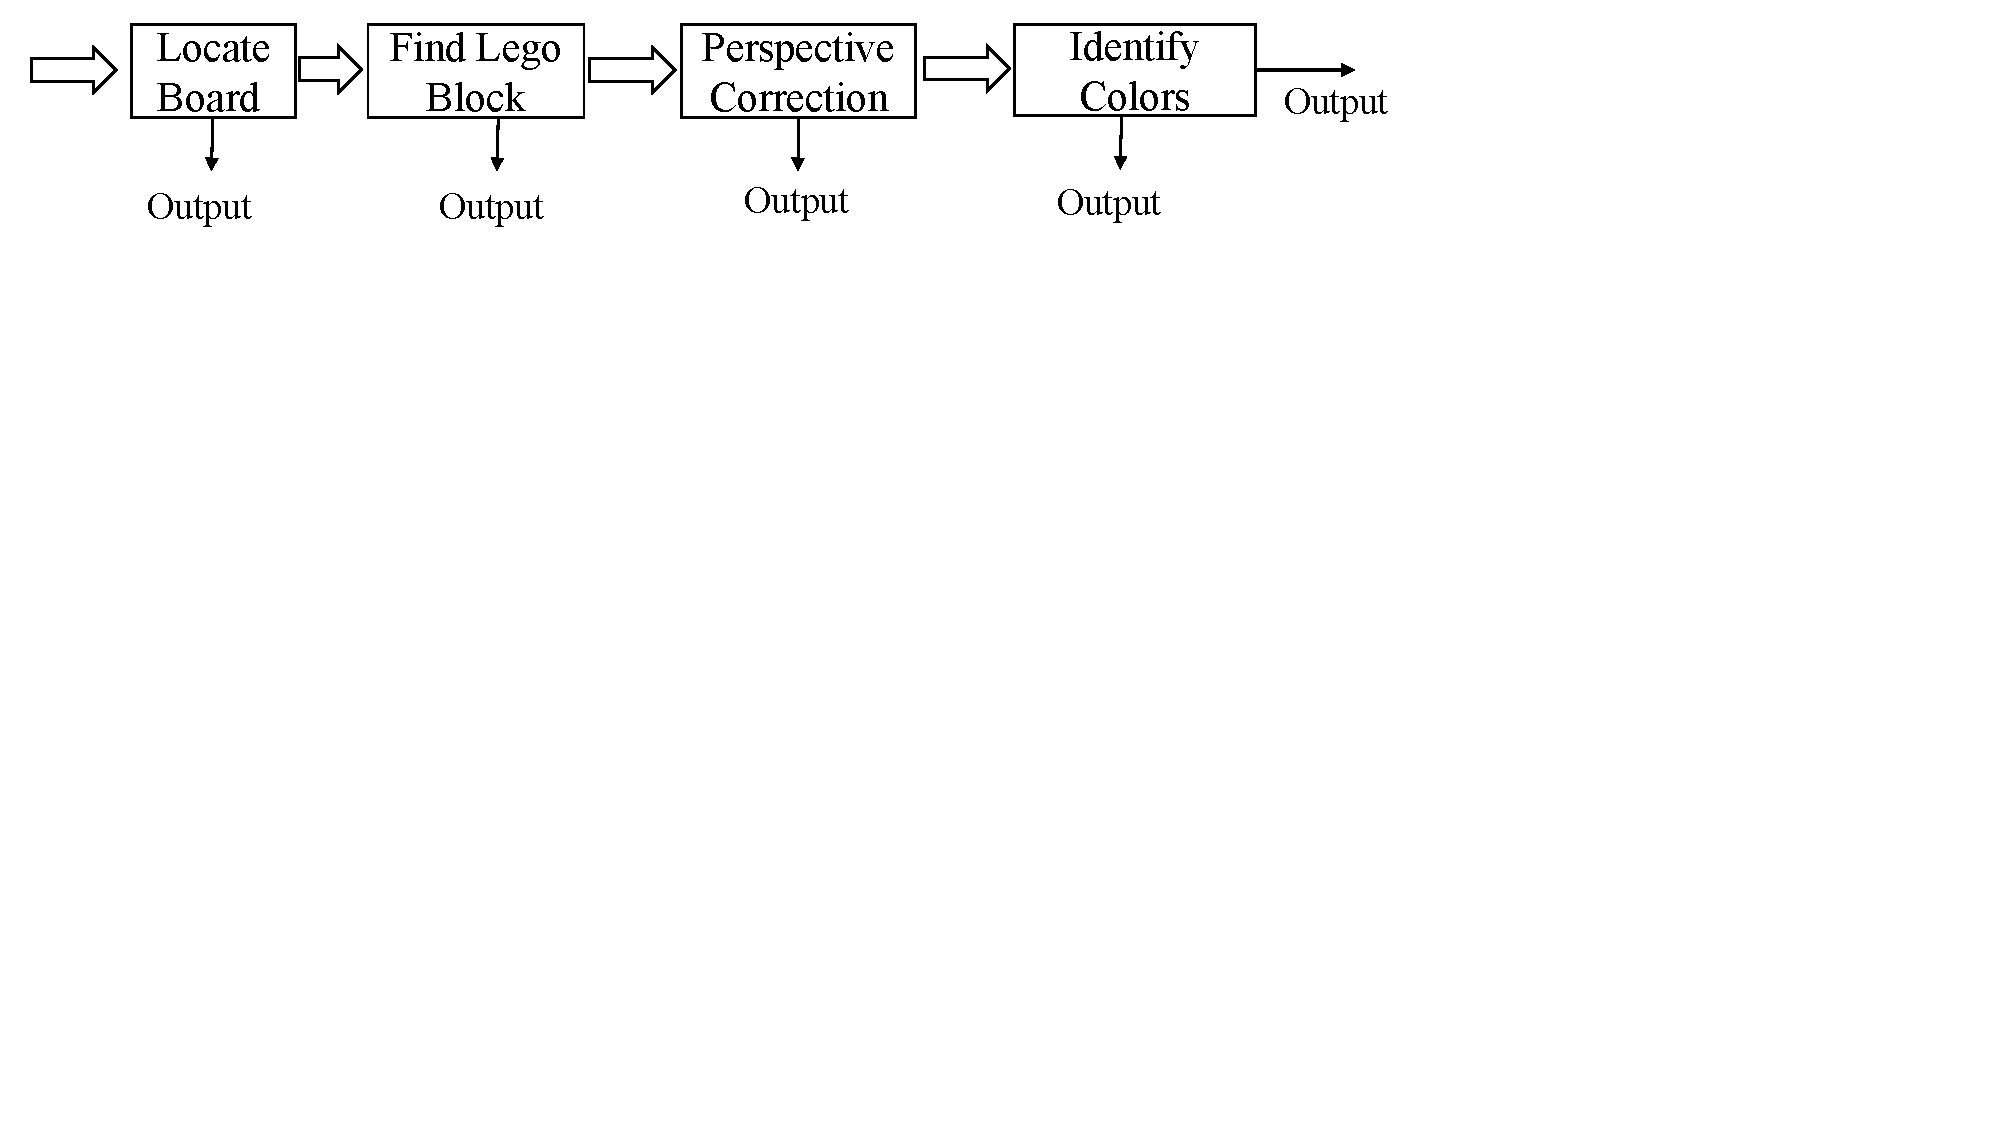
\includegraphics[width=\linewidth, trim=0em 30em 20em 0em,clip]{FIGS/fig-lego-dag.pdf}
\caption{LEGO Processing DAG}
\label{fig:lego-dag}
\end{figure}

To adequately provision resources for an application, one approach is
to leave the burden to developers, asking them to specify and reserve
a static amount of cores and memories needed for the service. However,
this method is known to be highly inaccurate and typically leads to
over-reservation in data-centers. For cloudlets, which are more
resource constrained, such over-reservation will lead to even worse
under-utilization or inequitable sharing of the available resources.
Instead, we seek to create an automated resource allocation system
that leverages knowledge of the application requirements and minimizes
developer effort.  To this end, we ask developers to provide target
Quality of Service (QoS) metrics or a utility function that relates a
single, easily-quantified metric (such as latency) to the quality of
user experience.  Building on this information, we construct offline
application profiles that map multidimensional resource allocations to
application QoS metrics.  At runtime, we calculate a resource
allocation plan to maximize a system-wide metric (e.g., total utility,
fairness) specified by cloudlet owner. We choose to consider the
allocation problem per application rather than per client in order to
leverage statistical multiplexing among clients and multi-user
optimizations (e.g., cache sharing) in an application.

\begin{figure}
\centering
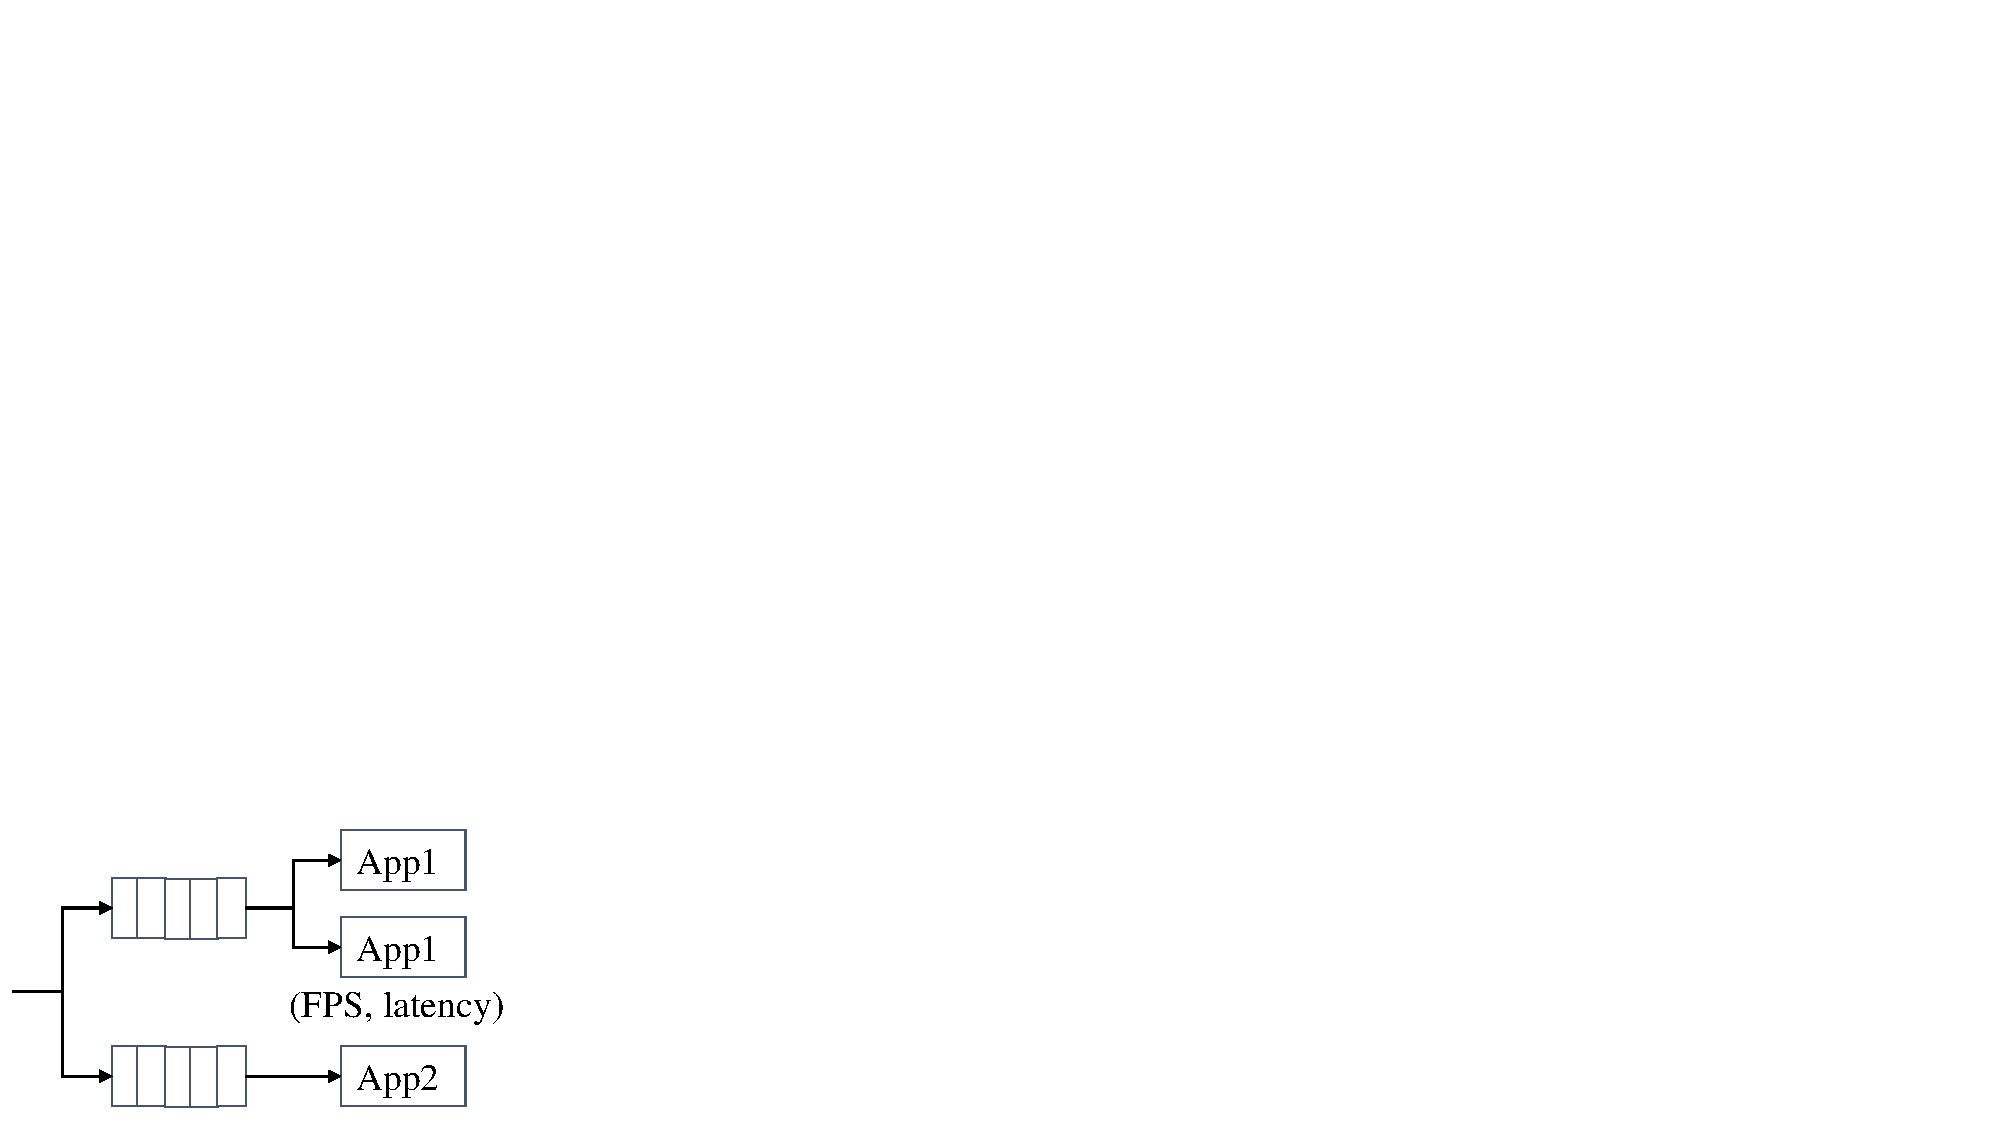
\includegraphics[width=0.5\linewidth]{FIGS/fig-allocation-system-model-cropped.pdf}
\begin{captiontext}Only request flow is shown.\end{captiontext}
\caption{Resource Allocation System Model}
\label{fig:allocation-system-model}
\vspace{-0.2in}
\end{figure}

\subsection{System Model}
Figure~\ref{fig:allocation-system-model} shows the system model we
consider. Each application is given a separate input queue. Each queue
can feed one or more application instances. Each application instance
is encapsulated in a container with controlled resources. In this
model, with adequate computational resources, clients of different
applications have minimal sharing and mainly contend for the wireless
network.

We use a utility-based approach to measure and compare system-wide
performance under different allocation schemes. For WCA, the utility
of a cloudlet response depends on both the quality of response and its
QoS characteristics (e.g., end-to-end latency). The total utility of a
system is the sum of all individual utilities. A common limitation of
a utility-based approach is the difficulty of creating these
functions. One way to ease such burden is to position an application
in the taxonomy described in Section~\ref{sec:taxonomy} and borrow
from similar applications. Another way is to calculate or measure
application latency bounds, such as through literature review or
physics-based calculation as done in~\cite{chen2017empirical}.

The system-wide performance is a function of the following independent
variables. 
\begin{enumerate}[label=(\alph*)]
    \item the number of applications and the number of clients of
each application;
    \item the number of instances of each application;
    \item the resource allocation for each instance;
\end{enumerate}

Although (a) is not under our control, Gabriel is free to adapt (b) and (c).
Furthermore, to optimize system performance, it may sacrifice the performance of
certain applications in favor of others. Alternatively, it may choose not to run
certain applications.


\begin{figure}
\centering
\begin{minipage}[b]{.35\linewidth}
\centering
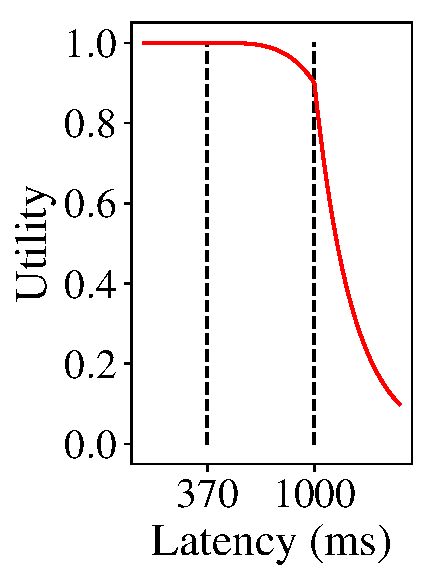
\includegraphics[width=\linewidth,trim=0em 0em 0em 0em, clip]{FIGS/fig-lat-util-face.pdf}
{(a) Utility For FACE}
\end{minipage}
\begin{minipage}[b]{.6\linewidth}
\centering
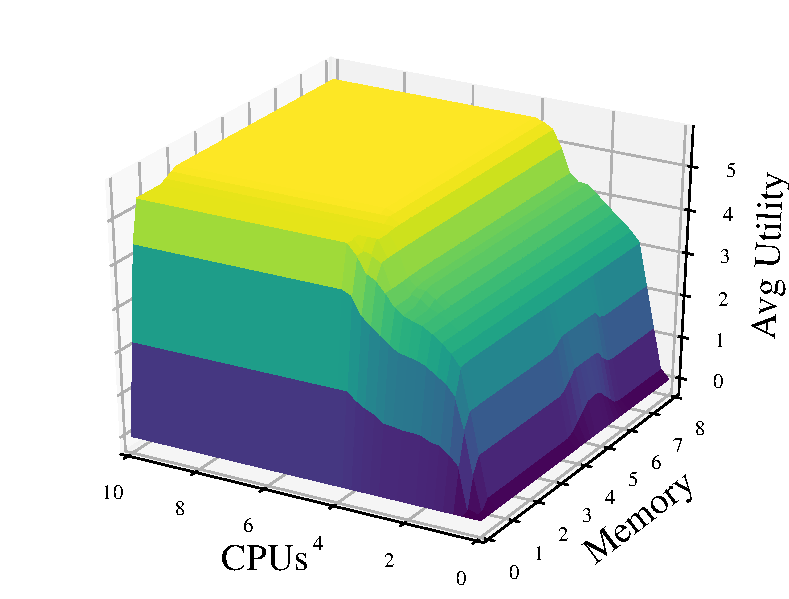
\includegraphics[width=\linewidth, trim=0em 0em 0em 0em, clip]{FIGS/fig-app-profile-face.pdf}
{(b) Profile for FACE}
\end{minipage}
\caption{FACE Application Utility and Profile}
\label{fig:face-utility-and-profile}
\end{figure}

\begin{figure}
\centering
\begin{minipage}[b]{.35\linewidth}
\centering
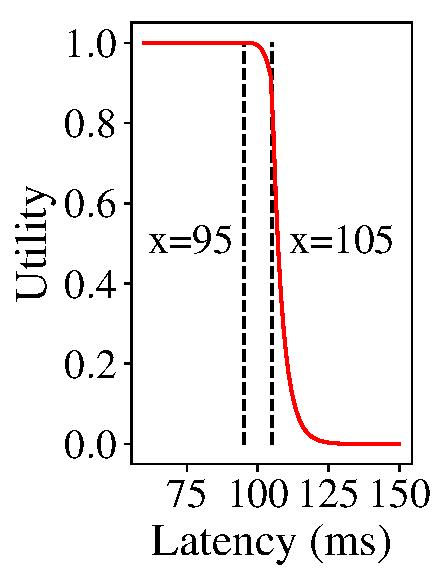
\includegraphics[width=\linewidth,trim=0em 0em 0em 0em, clip]{FIGS/fig-lat-util-pool.pdf}
{(a) Utility For POOL}
\end{minipage}
\begin{minipage}[b]{.6\linewidth}
\centering
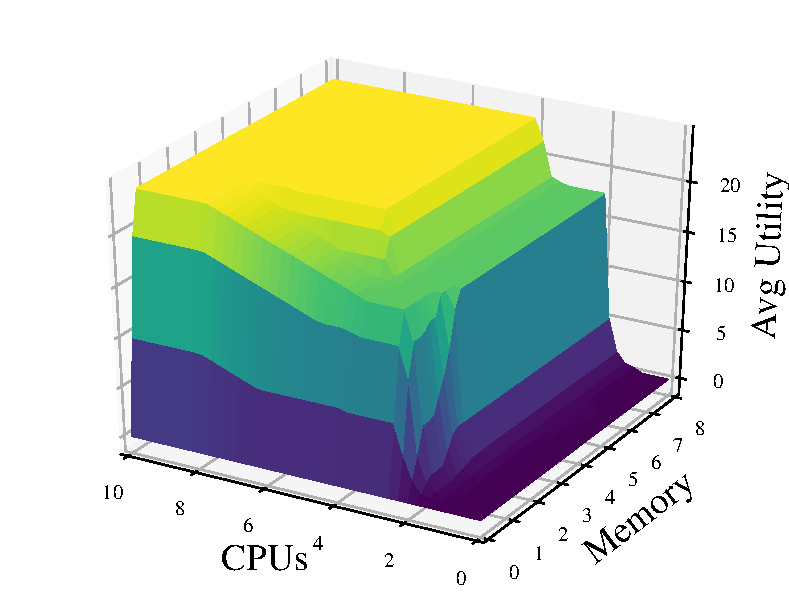
\includegraphics[width=\linewidth, trim=0em 0em 0em 0em, clip]{FIGS/fig-app-profile-pool.pdf}
{(b) Profile for POOL}
\end{minipage}
\caption{POOL Application Utility and Profile}
\label{fig:pool-utility-and-profile}
\end{figure}

\subsection{Application Utility and Profiles}

We build application profiles offline in order to estimate latency and
throughput at runtime. First, we ask developers to provide a utility
function that maps QoS metrics to application experience.
Figure~\ref{fig:face-utility-and-profile}(a) and
Figure~\ref{fig:pool-utility-and-profile}(a) show utility functions
for two applications based on latency bounds identified
by~\cite{chen2017empirical} for each request. Next, we profile an application
instance by running it under a discrete set of cpu and memory
limitations, with a large number of input requests. We record the
processing latency and throughput, and calculate the system-wide
utility per unit time. We interpolate between acquired data points of
(system utility, resources) to produce continuous functions.  Hence,
we effectively generate a multidimensional resource to utility profile
for each application.

We make a few simplifying assumptions to ensure profile generation and
allocation of resources by utility are tractable.  First, we assume utility
values across different applications are comparable. Furthermore, we assume
utility is received on a per-frame basis, with values that are normalized
between 0 and 1.  Each frame that is sent, accurately processed, and replied
within its latency bound receives 1, so a client running at 30 FPS under ideal
conditions can receive a maximum utility of 30 per second.  This clearly ignores
variable utility of processing particular frames (e.g., differences between
active and passive phases), but simplifies construction of profiles and modeling
for resource allocation; we leave the complexities of variable utility to future
work. Figure~\ref{fig:face-utility-and-profile}(b) and
Figure~\ref{fig:pool-utility-and-profile}(b) show the generated application
profiles for FACE and POOL. We see that POOL is more efficient than FACE in
using per unit resource to produce utility. If an application needs to deliver
higher utility than a single instance can, our framework will automatically
launch more instances of it on the cloudlet.
